\chapter{Specyfikacja zewnętrzna}
\label{ch:04}

\section{Wygląd interfejsu użytkownika}

\note{Ta część powinna zawierać screeny z interfejsem użytkownika wraz z porównaniem do projektu graficznego.}

\begin{figure}[H]
    \centering
    \begin{subfigure}{0.40\textwidth}
        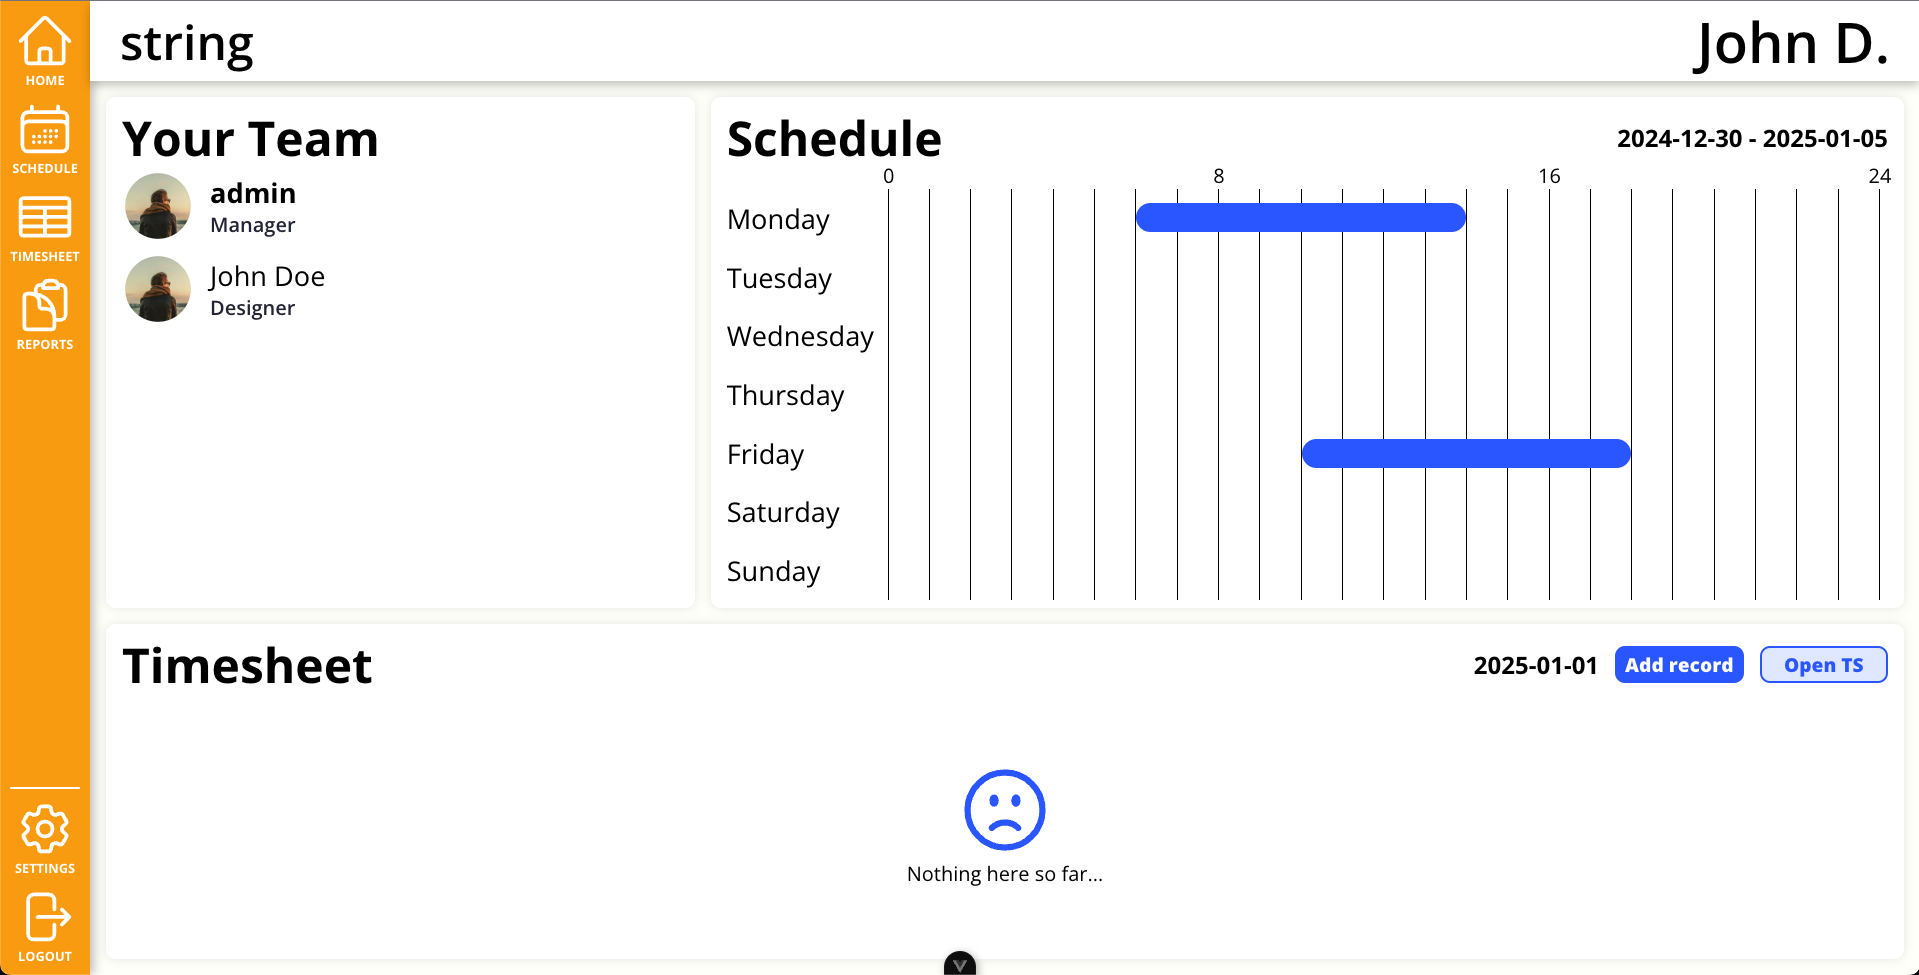
\includegraphics[width=\textwidth]{graf/userDashboard.png}
        \caption{Panel użytkownika}
        \label{fig:userDashboard}
    \end{subfigure}
    \begin{subfigure}{0.40\textwidth}
        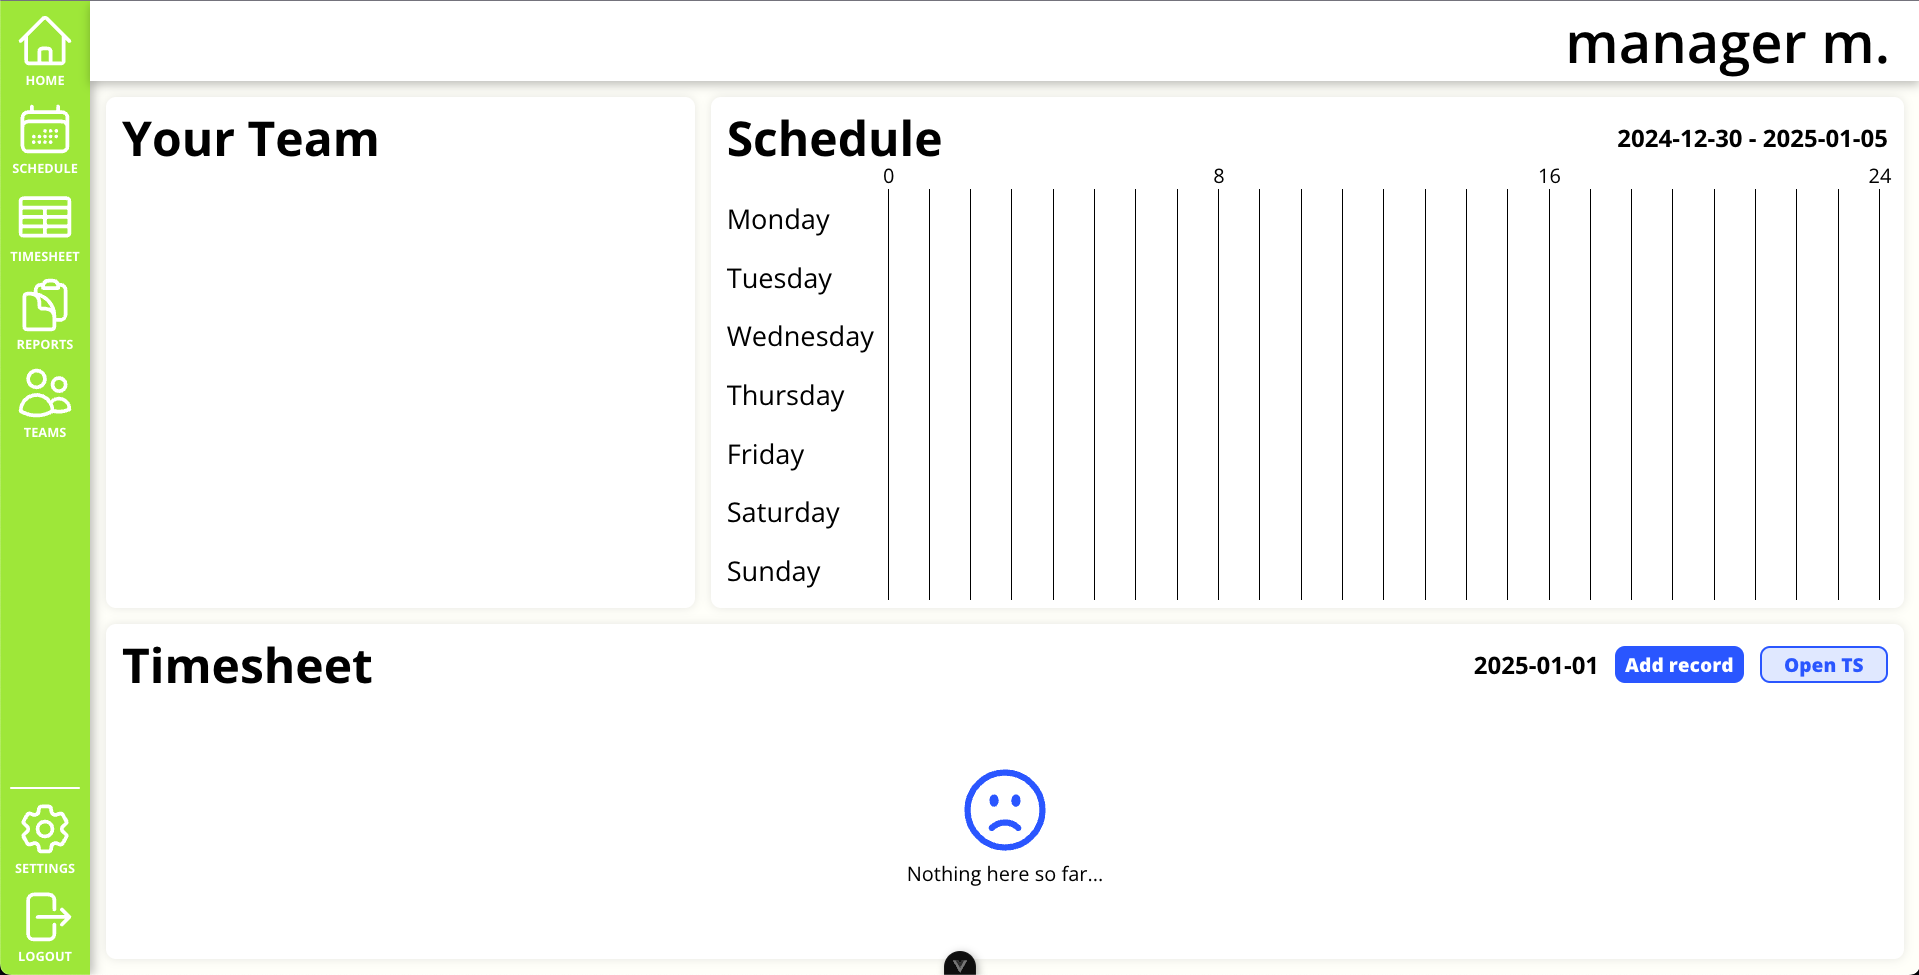
\includegraphics[width=\textwidth]{graf/managerDashboard.png}
        \caption{Panel managera}
        \label{fig:managerDashboard}
    \end{subfigure}
    \begin{subfigure}{0.40\textwidth}
        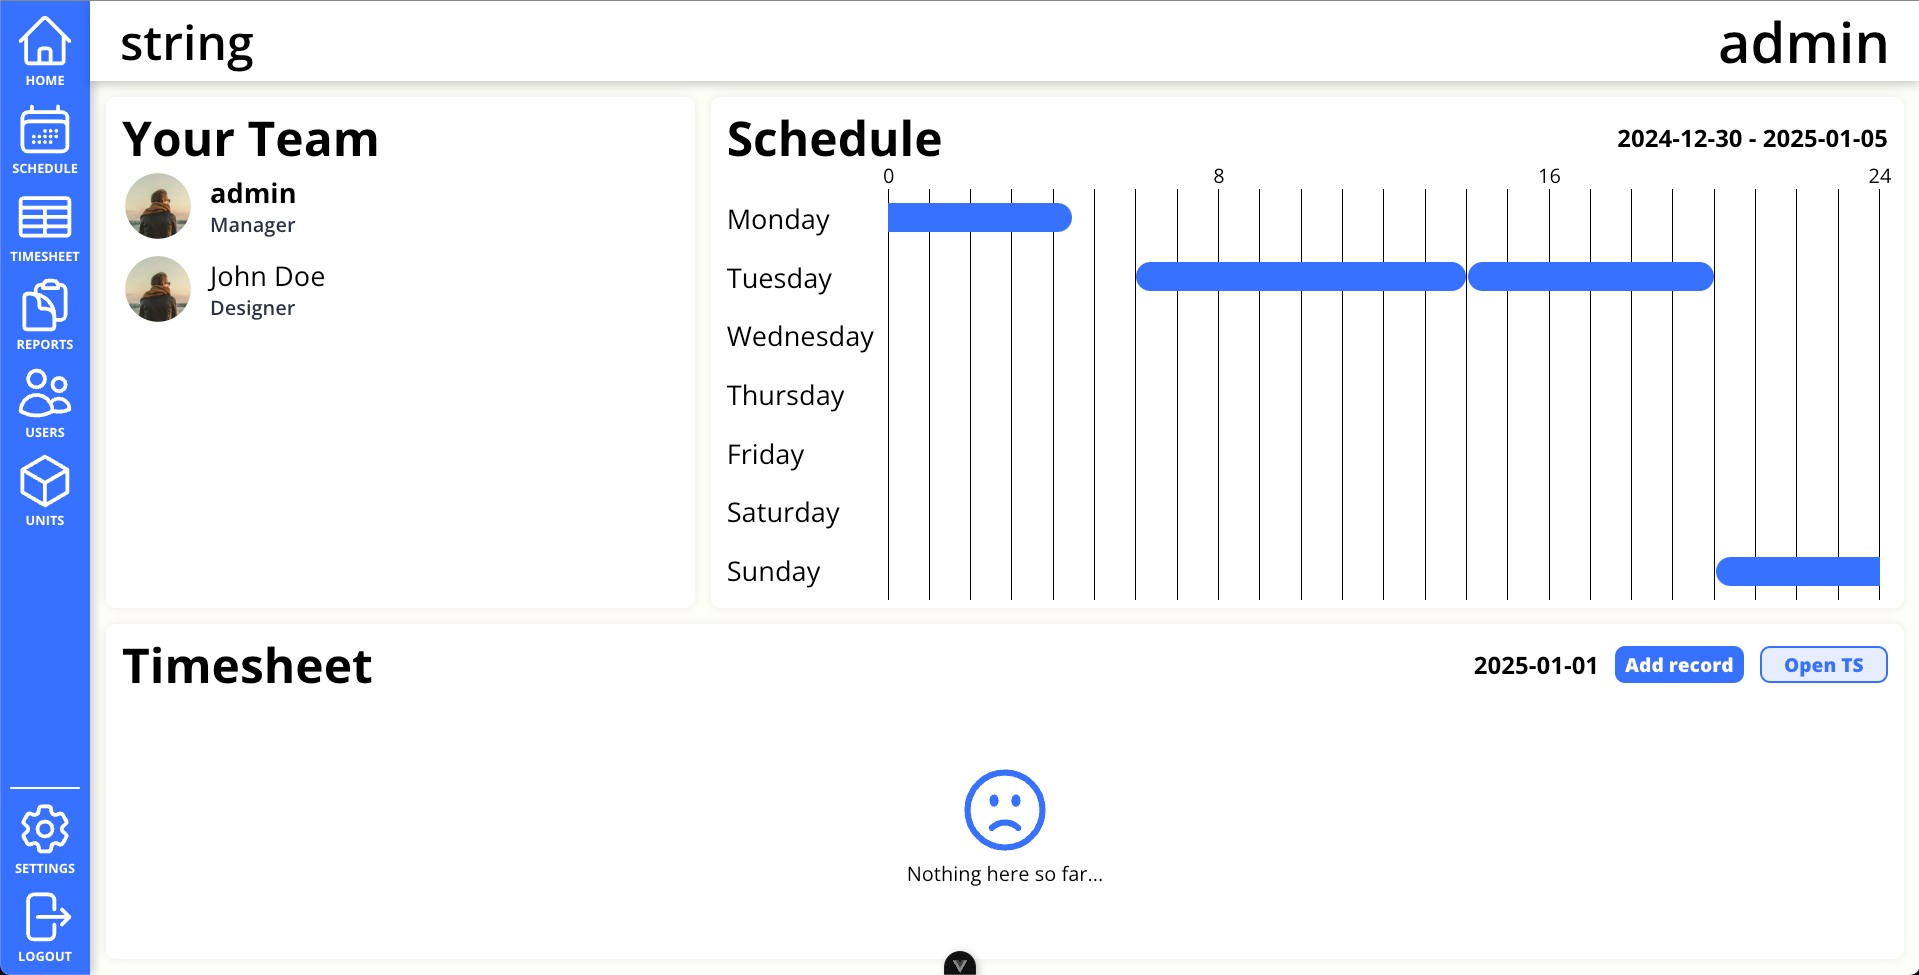
\includegraphics[width=\textwidth]{graf/adminDashboard.png}
        \caption{Panel administratora}
        \label{fig:adminDashboard}
    \end{subfigure}
    \caption{Panel główny}
    \label{fig:dashboard}
\end{figure}

\section{Użytkownicy i ich role}

W systemie zostały zdefiniowane 3 role użytkowników:

\begin{itemize}
    \item Użytkownik,
    \item Manager,
    \item Administrator.
\end{itemize}

Dodatkowo każde konto użytkownika może zostać zarchiwizowane, co oznacza, że użytkownik nie ma dostępu do systemu, ale jego dane pozostają w bazie danych.

Każda rola posiada inne uprawnienia i możliwości w systemie. Role można bardzo łatwo od siebie odróżnić, ponieważ każda z nich posiada inny kolor widoczny na pasku nawigacyjnym. Poniżej zostały przedstawione informacje na temat każdej z nich.

\subsection{Użytkownik}

\textbf{Użytkownik} jest podstawową rolą w systemie. Posiada możliwość przeglądania swoich danych, harmonogramu pracy, oraz dodawania wpisów do timesheetu. Użytkownik nie ma możliwości zarządzania innymi użytkownikami, ani zmiany ustawień systemu.

Kolorem przypisanym do użytkownika jest kolor pomarańczowy:
\begin{itemize}
    \item \texttt{\#FCAB10},
    \item \texttt{rgb(252, 171, 16)},
    \item \texttt{hsl(39, 98\%, 53\%)}.
\end{itemize}

\subsection{Manager}

\textbf{Manager} jest rolą posiadającą większe uprawnienia niż użytkownik. Oprócz możliwości przeglądania swoich danych, harmonogramu pracy, oraz dodawania wpisów do timesheetu, manager może również zarządzać przypisanym do siebie zespołem, harmonogramem pracy zespołu oraz przeglądać i akceptować timesheety swoich pracowników. Manager nie ma możliwości zarządzania innymi managerami.

Kolorem przypisanym do managera jest kolor zielony:
\begin{itemize}
    \item \texttt{\#ACE849},
    \item \texttt{rgb(172, 232, 73)},
    \item \texttt{hsl(79, 73\%, 61\%)}.
\end{itemize}

\subsection{Administrator}

\textbf{Administrator} jest użytkownikiem o największych uprawnieniach w systemie. Rozszerza możliwości managera o możliwość zarządzania poszczególnymi użytkownikami i ich rolami, strukturą organizacyjną firmy - dodawanie, edycję i usuwanie działów oraz stanowisk - oraz konfigurację systemu. Administrator ma dostęp do wszystkich danych w systemie.

Kolorem przypisanym do administratora jest kolor niebieski:
\begin{itemize}
    \item \texttt{\#3772FF},
    \item \texttt{rgb(55, 114, 255)},
    \item \texttt{hsl(219, 79\%, 59\%)}.
\end{itemize}

\note{Ta część mogła by być opisana przy projektowaniu systemu.}

\section{Dostępność}

\subsection{Dostępność cyfrowa}

Aplikacja została zaprojektowana w taki sposób, aby możliwe było korzystanie z niej wyłącznie przy użyciu klawiatury. Użycie biblioteki komponentów \texttt{PrimeVue} pozwoliło na zapewnienie dostępności dla osób o ograniczonych możliwościach ruchowych. Komponenty umieszczone na stronie internetowej są zgodne z wytycznymi \texttt{WCAG 2.1}. \cite{bib:WCAG21}

\subsection{Dostępność językowa}

W celu zapewnienia dostępności systemu użytkownikom z różnych krajów i regionów, aplikacja dostarcza możliwość zmiany języka interfejsu użytkownika. W chwili obecnej dostępne są 2 języki: polski i angielski, jednakże dodanie kolejnego nie wymaga od programisty dużego nakładu pracy. Każdy z języków jest przechowywany w oddzielnym pliku \texttt{.json}, co pozwala na jego łatwą modyfikację lub dodanie nowego. Część pliku zawierającego tłumaczenia na język polski została przedstawiona na rysunku \ref{lst:pl}.

\begin{figure}[H]
    \begin{minted}[linenos,breaklines,frame=lines]{json}
"form": {
    "save": "Zapisz",
    "cancel": "Anuluj",
    "fieldRequired": "To pole jest wymagane",
    "invalidFormat": "Nieprawidłowy format"
},
\end{minted}
    \caption{Fragment pliku z tłumaczeniami na język polski}
    \label{lst:pl}
\end{figure}